\begin{figure}[htbp]
\section*{ STXBP1}
\centering
\begin{subfigure}[b]{0.95\textwidth}
\centering
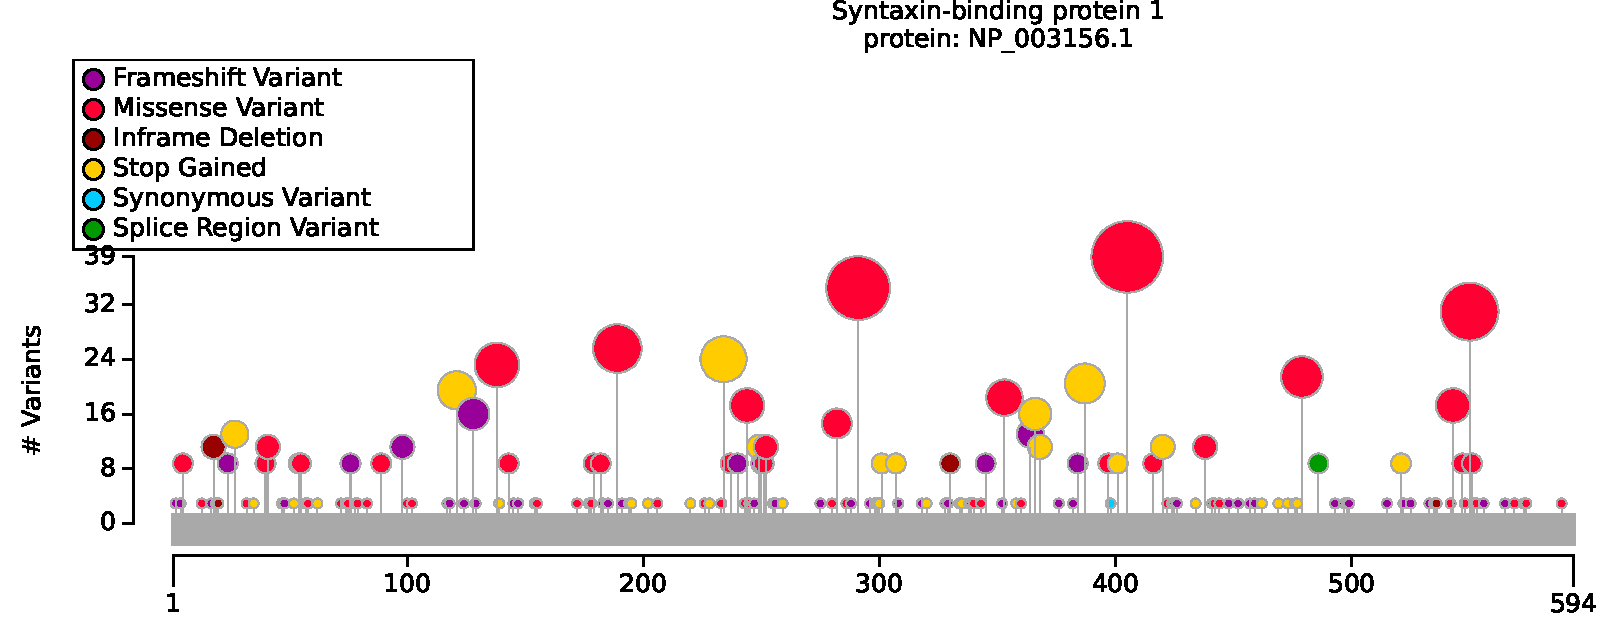
\includegraphics[width=\textwidth]{ img/STXBP1_protein_diagram.pdf} 
\captionsetup{justification=raggedright,singlelinecheck=false}
\caption{Distribution of variants in STXBP1}
\end{subfigure}

\vspace{2em}

\begin{subfigure}[b]{0.95\textwidth}
\centering
\resizebox{\textwidth}{!}{
\begin{tabular}{llllrr}
\toprule
Genotype (A) & Genotype (B) & total tests performed & significant results\\
\midrule
Missense & Other & 18 & 0\\
Arg406 Variants & Other & 18 & 0\\
Exon 14 & Other & 18 & 0\\
\bottomrule
\end{tabular}
}
\captionsetup{justification=raggedright,singlelinecheck=false}
\caption{Fisher Exact Test performed to compare HPO annotation frequency with respect to genotypes. }
\end{subfigure}

\vspace{2em}

\caption{ The cohort comprised 462 individuals (206 females, 220 males, 36 with unknown sex). A total of 516 HPO terms were used to annotate the cohort. Disease diagnosis: Developmental and epileptic encephalopathy 4 (OMIM:612164). No significant genotype-phenotype correlations identified. A total of 259 unique variant alleles were found in \textit{STXBP1} (transcript: \texttt{NM\_003165.6}, protein id: \texttt{NP\_003156.1}).}
\end{figure}
